\section{Introduction}

\subsection{General Characteristics}
As the jet era started, Sweden foresaw the need for a jet fighter that could intercept bombers at high 
altitude and also successfully engage fighters. Although other interceptors such as the 
US Air Force's F-104 Starfighter were being conceived during the same period, 
Saab's "Draken" would have to undertake a combat role unique to Sweden. 
Other demanding requirements were the capability to operate from reinforced public roads 
used as part of wartime airbases, and for refuelling/rearming to be 
carried out in no more than ten minutes, by conscripts with minimal training. 
\textbf{In September 1949, the Swedish Defence Material Administration issued a request for a fighter/interceptor aircraft, and work began at Saab the same year}

\textit{Regarding the aerodynamic design of the J35 Draken the two major options were swept wings and delta wings.}
The question was quickly resolved by the initial studies which had called for the
exploration of a swept wing configuration. In short order it  was determined tha
in consideration of all other parameteres placed upon the design, 
the swept wing's aerodynamic drag at high Mach numbers was too high, 
and its configuration requirements dictated that the fuselage have insufficient 
volume for equipment, fuel and armament.
The Delta wing on the other hand showed great promise following initial tunnel 
tests. The pure delta soon was ruled out, however, as it suffered from center 
of gravity and center of pressure anomalies that were difficult to alleviate. 
A derivative, however, often referred to as \textit{the double delta}, proved much more flexible. 
In general the double delta was found to offer the attributes of:
\begin{itemize*}
    \item reduced frontal area while permitting optimal wing area
    \item More favorable wing sweep angles on the center wing section
    \item Center of gravity and center of pressure being closer to each other
    \item More favorable area distribution
    \item Low supersonic drag
    \item Favorable low speed drag
    \item Strong and stiff fail safe structure
    \item Being able to place the air intakese farther forward
\end{itemize*}
The double-delta configuration was first tested on the SAAB 210 which first flew
on 21 January 1952.

\begin{figure}[H]
  \centering
  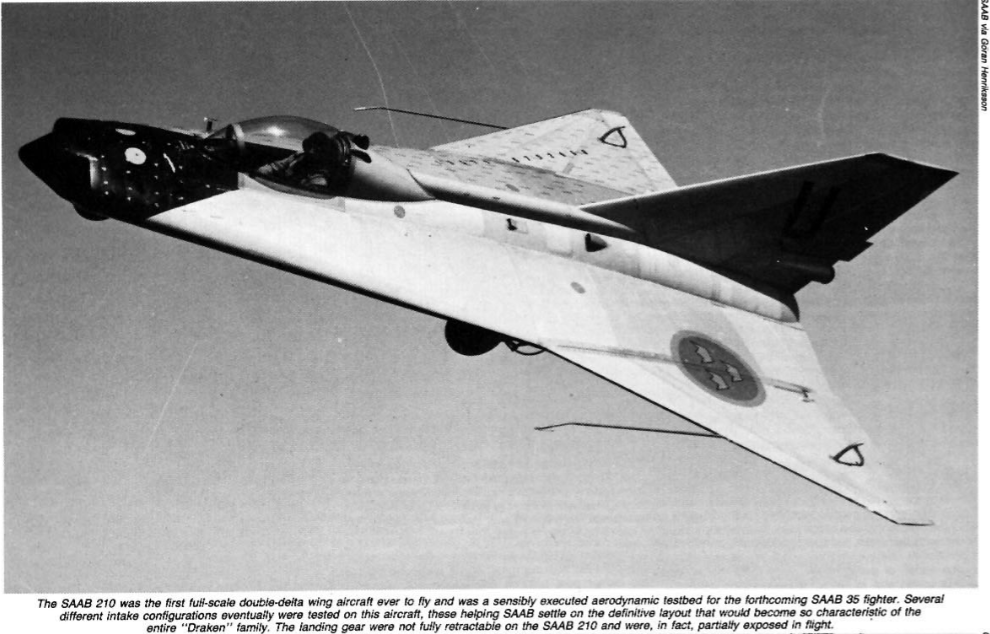
\includegraphics[width=1.2\textwidth]{SAAB210}
  \caption{SAAB 210}
\end{figure}
\begin{figure}[H]
  \centering
  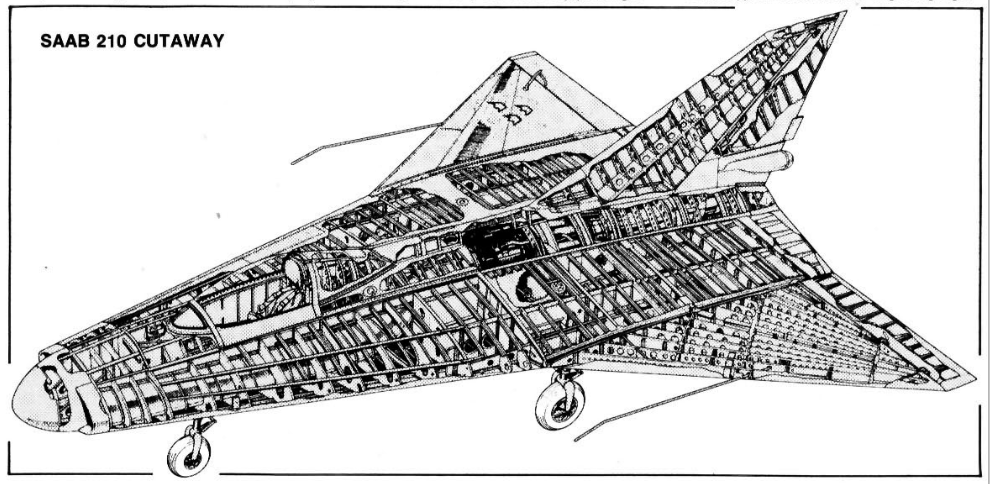
\includegraphics[width=1.3\textwidth]{Cutaway}
  \caption{Cutaway design of SAAB 210}
\end{figure}

\subsection{Basic Versions}

Below are the major versions of J35 Draken which were manufactured from 1955
to 1974 by Saab.
\subsubsection{J35A}

    \begin{itemize*}
        \item First flew on 1958
        \item Total Production: 90
        \item Delivered from 1959 to 1961
    \end{itemize*}

\begin{figure}[H]
  \centering
  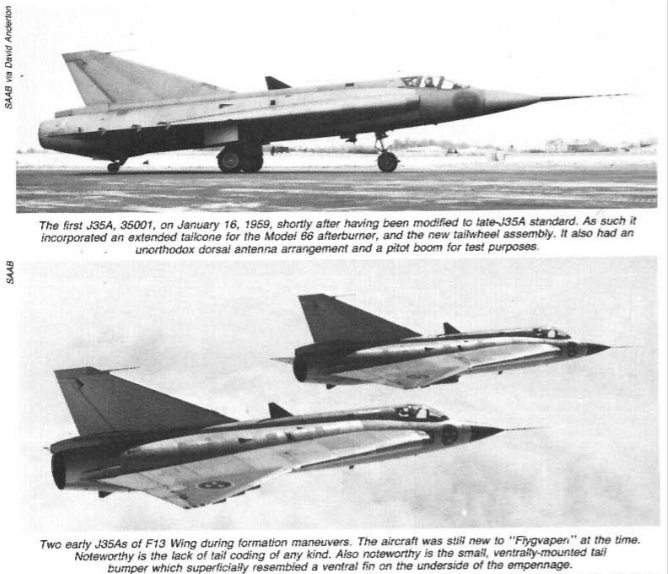
\includegraphics[width=1.0\textwidth]{J35A}
  \caption{J35A}
\end{figure}
\subsubsection{J35B}
\begin{itemize*}
        \item First flew on 1959
        \item Total Production: 73
        \item Delivered from 1962 to 1963
        \item First truly operating interceptor version of J35 Draken
    \end{itemize*}

\begin{figure}[H]
    \centering
    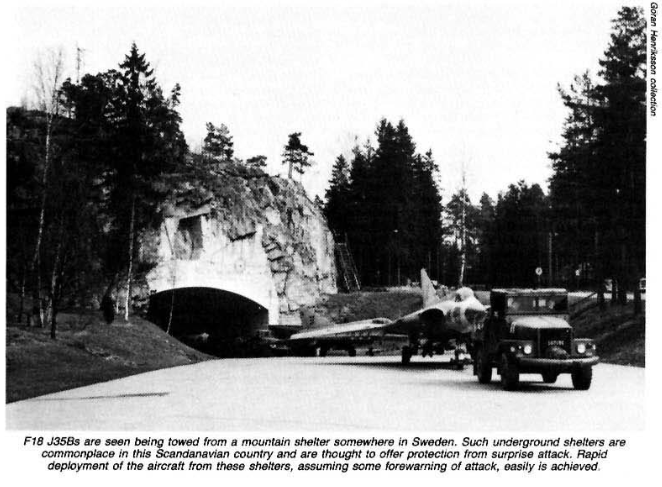
\includegraphics[width=1.0\textwidth]{S35b_sheltered}
    \caption{J35B carried out of sheltered area}
\end{figure}

\begin{figure}[H]
    \centering
    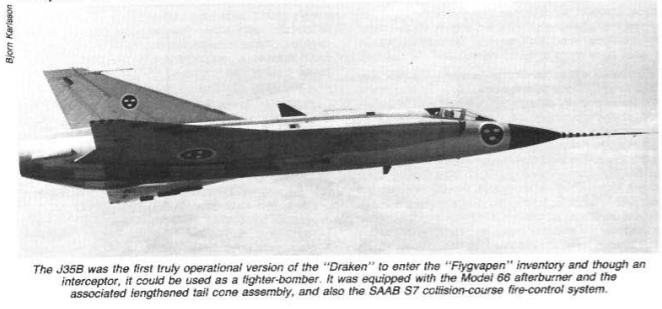
\includegraphics[width=1.0\textwidth]{S35B}
    \caption{J35B}
\end{figure}

\subsubsection{Sk35C}
    \begin{itemize*}
        \item First flew on 1959
        \item Total Production: -
        \item Essentially 25 J35A with short tail sections rebuilt 
            into a twin-seated trainer version
        \item To provide space for a second cockpit some equipment was relocated and the size of the forward
            fuel tank was reduced.
        \item Lacking the guns and radar of single-seater, the Sk35C nevertheless could be 
            used for armament training with Sidewinder missiles and other external stores.
    \end{itemize*}

\begin{figure}[H]
  \centering
  \hspace*{-2cm} 
  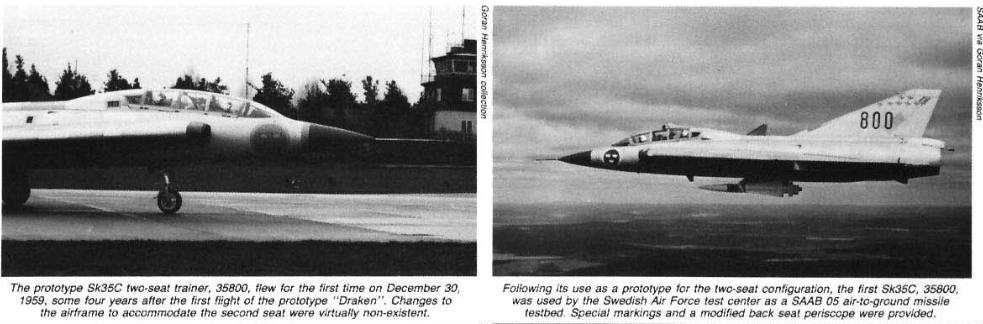
\includegraphics[width=1.2\textwidth]{Sk35C}
  \caption{Sk35C}
\end{figure}

\subsubsection{J35D}
    \begin{itemize*}
        \item First flew on 1960
        \item Total Production: 120
        \item Delivered from 1963 to 1964
        \item Fastest Draken version, capable of accelerating until out of fuel.
        \item Represented a marked improvement over earlier versions both in terms of performance and combat capabillities.
            The former was obtained by replacing the RM5B engine with RM5C (Avon-300 series) thus increasing the max thrust forom 6.850 kgp to 7.750 kgp
            when using the afterburner.
    \end{itemize*}

\begin{figure}[H]
  \centering
  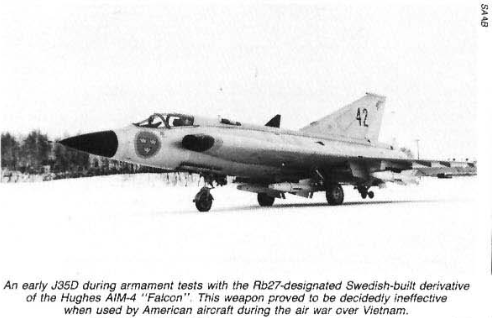
\includegraphics[width=1.0\textwidth]{J35D}
  \caption{J35D}
\end{figure}

\subsubsection{S35E}
    \begin{itemize*}
        \item Total Production: 60
    \end{itemize*}


\begin{figure}[H]
    \centering
    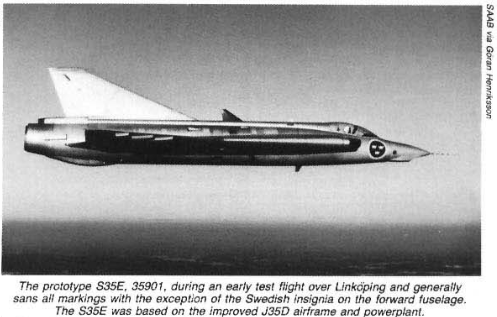
\includegraphics[width=\textwidth]{S35E}
    \caption{J35E}
\end{figure}
\begin{figure}[H]
    \centering
    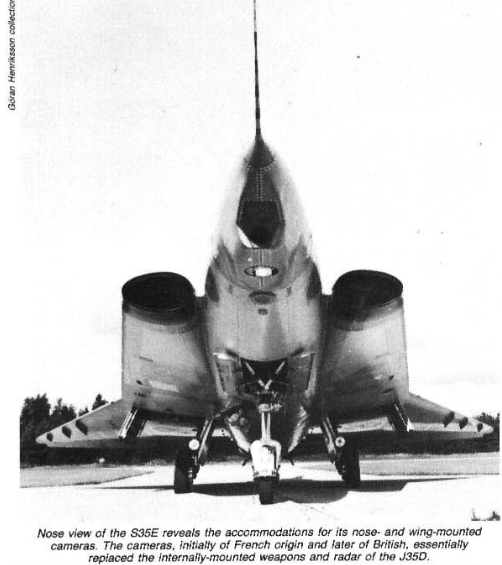
\includegraphics[width=\textwidth]{S35E_b}
    \caption{J35E nose view}
\end{figure}

\subsubsection{S35F}
\begin{figure}[H]
    \centering
    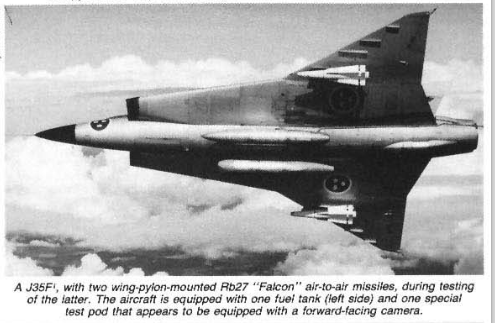
\includegraphics[width=\textwidth]{S35F}
    \caption{J35F}
\end{figure}
\begin{figure}[H]
    \centering
    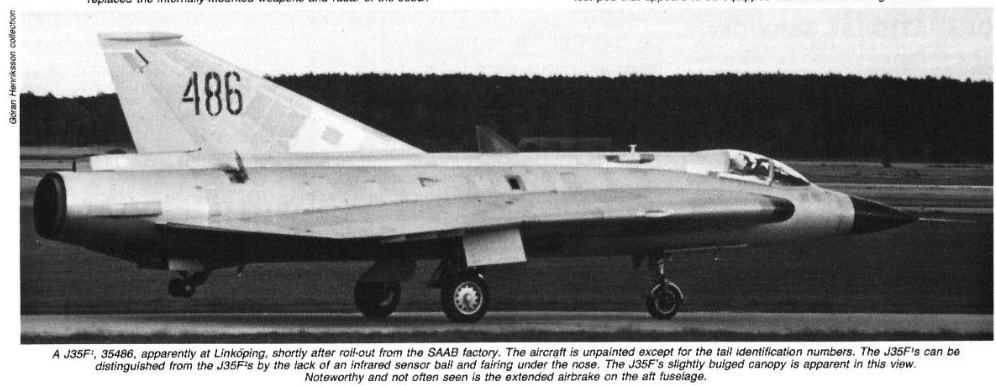
\includegraphics[width=\textwidth]{S35F_b}
    \caption{J35F landing}
\end{figure}

\subsubsection{S35H}
Version of J35 which was supposed to be sold to Switzerland by SAAB. During 1960 it 
was evaluated thoroughly in Switzerland with generally favorable results.
The J35H was not however the only aircraft considered and in the end the Schweizerische
Fliegertruppe concluded that a slightly modified version of Dassault Mirage III was more ideally suited.

\subsubsection{SAAB 35XD}
\begin{itemize*}
    \item Company designation in which X stoood for export and D for Denmark
    \item In 1968 The Danish Goverment ordered 20 single seated 3 two seated trainers 
        23 photo-reconnaissance aircrafts in a follow up order. Finally the Danes revised their offer for 20 single seat 
        20 reconnaisance aircrafts and 11 two-seat trainers.
\end{itemize*}

\subsubsection{SAAB 35XS}
\begin{itemize*}
    \item Export version for Suomi or Finland
    \item Ordered during 1970 by Finland
\end{itemize*}
